% das Papierformat zuerst
\documentclass[a4paper, 11pt]{article}
\usepackage[margin=3cm]{geometry}
\usepackage[utf8]{inputenc}
\usepackage[T1]{fontenc}
\usepackage[ngerman]{babel}
\usepackage{hyperref} % clickable refs
\usepackage{graphicx}
\usepackage[toc, numberedsection]{glossaries}
\usepackage{float}

\makeglossary

%Hack for referencing labels
\makeatletter
\def\namedlabel#1#2{\begingroup
    #2%
    \def\@currentlabel{#2}%
    \phantomsection\label{#1}\endgroup
}
\makeatother
% End: Hack for referencing labels

% Glossar: alle Einträge, aber ohne extra Referenzen
% http://tex.stackexchange.com/questions/115635/glossaries-suppress-pages-when-using-glsaddall
\newcommand*{\glsgobblenumber}[1]{}
\makeatletter
\newcommand*{\glsaddnp}[2][]{
  \glsdoifexists{#2}{
    \def\@glsnumberformat{glsgobblenumber}
    \edef\@gls@counter{\csname glo@#2@counter\endcsname}
    \setkeys{glossadd}{#1}
    \@gls@saveentrycounter
    \@do@wrglossary{#2}
  }
}
\newcommand{\glsaddallunused}[1][]{
  \edef\@glo@type{\@glo@types}
  \setkeys{glossadd}{#1}
  \forallglsentries[\@glo@type]{\@glo@entry}{
    \ifglsused{\@glo@entry}{}{
      \glsaddnp[#1]{\@glo@entry}}}
}
\makeatother

\renewcommand{\glsnamefont}[1]{\mdseries #1} % glossary entries shouldn’t be bold

% Glossar

% So sieht ein Glossar-Eintrag aus:
%
%\newglossaryentry{dijkstra}{
%  name={Dijkstra’s Algorithmus},
%  description={ein Algorithmus, um den optimalen Pfad in einem gerichteten Graphen zu finden}
%}
%\newglossaryentry{arc}{
%  name={Arc-Flags},
%  description={eine Technik, um Routenberechnung zu beschleunigen},
%  see={dijkstra}
%}
%
% Und so kann er im Dokument verwendet werden:
%
% lorem ipsum dolor sit \gls{arc}, consectetur
%
% End: Glossar

% usage: \counteditem{prefix}{refName} -> item `/prefixXX/` with label `prefix:refName` (where XX is counted in increments of 10)
\makeatletter
\newcommand{\oitem}[2]{
  % define the counter
  \@ifundefined{c@oitem#1}{\newcounter{oitem#1}}{} % initialized at 0
  \addtocounter{oitem#1}{10}
  \item[\namedlabel{#1:#2}{/#1\arabic{oitem#1}/}]
}
\makeatother

% usage: \testfall{szenario}{ablauf}{ergebnis} oder \testfall[\ref{F:getesteteFunktion}]{szenario}{ablauf}{ergebnis}
\newcommand{\testfall}[4][]{
  \begin{description}
    \ifthenelse{\equal{#1}{}}
               {} % optional argument #1 is empty: skip
               {\item[Testet] #1}
    \item[Vorbedingungen] #2
    \item[Ablauf] #3
    \item[Erwartetes Ergebnis] #4
  \end{description}
}

% Betreuer: Rand reduzieren. (gemacht)
% Betreuer: Wichtig, viel Kriterien, GUI, Testfälle (gemacht)
% Betreuer: Präzise!!! (gemacht)
%TODO Programm/Software => routeKIT wo angebracht (gemacht)
% hier beginnt das Dokument (oder auch nicht)
\begin{document}
\shorthandoff{"}

% place a symbol before clickable links
% this has to come *after* \begin{document} because hyperref installs a \AtBeginDocument hook that updates the ref command.
\newcommand{\refsymbol}[0]{\scalebox{0.5}{$\nearrow$}}
\let\oldref\ref
\renewcommand{\ref}[1]{\refsymbol\oldref{#1}}
\let\oldgls\gls
\renewcommand{\gls}[1]{\refsymbol\oldgls{#1}}
\let\oldGls\Gls
\renewcommand{\Gls}[1]{\refsymbol\oldGls{#1}}
\let\oldglslink\glslink
\renewcommand{\glslink}[2]{\refsymbol\oldglslink{#1}{#2}}
\let\oldhyperref\hyperref
\renewcommand{\hyperref}[2][notActuallyOptional]{\refsymbol\oldhyperref[#1]{#2}}
\let\oldautoref\autoref
\renewcommand{\autoref}[1]{\refsymbol\oldautoref{#1}}

\newcommand{\abbildung}[1]{\autoref{fig:#1}}

% Betreuer: Berechnung von Punkt auf Kante zu Punkt auf Kante.  (KdBaum über Kanten) (gemacht)
% Betreuer: Profile exakt welcher Typ (gemacht)

% alle Glossareintraege
\newacronym[longplural=Personenkraftwagen]{pkw}{PKW}{Personenkraftwagen}
\newacronym[longplural=Lastkraftwagen]{lkw}{LKW}{Lastkraftwagen}
\newacronym{osm}{OSM}{OpenStreetMap}
\newacronym{gui}{GUI}{Graphical User Interface}
\newacronym[longplural={Points of interest}]{poi}{POI}{Point of interest}
\newacronym{gpx}{GPX}{GPS Exchange Format}

\newglossaryentry{profil}{
  name={Profil},
  description={Enthält für die Routenplanung relevante Informationen, z.B. die Höhe und das Gewicht des Fahrzeugs},
  plural={Profile}
}
\newglossaryentry{osmkachel}{
  name={OSM-Kachel},
  description={Die öffentlichen gerenderten \gls{osm}-Kacheln z.B. auf \mbox{\url{http://a.tile.openstreetmap.org/}}},
  plural={OSM-Kacheln}
}
\newglossaryentry{route}{
  name={Route},
  description={Ein Weg zwischen zwei Punkten auf je einem Wegstück}
}
\newglossaryentry{rendern}{
  name={rendern},
  description={Berechnung eines Bilds aus den zu rendernden Daten}
}
\newglossaryentry{schnellroute}{
  name={schnellste Route},
  description={die \gls{route} mit der geschätzt kürzesten Fahrzeit}
}
\newglossaryentry{wegbeschreibung}{
  name={Wegbeschreibung},
  description={Beschreibung einer \gls{route} durch eine Liste von Abbiegeanweisungen}
}
\newglossaryentry{dijkstra}{
  name={Dijkstra’s Algorithmus},
  description={ein Algorithmus, um den optimalen Pfad in einem gerichteten Graphen zu finden}
}
\newglossaryentry{arc}{
 name={Arc-Flags},
 description={eine Technik, um Routenberechnung zu beschleunigen}
}
\newglossaryentry{beschleunigung}{
 name={Beschleunigung},
 description={Ermöglicht eine schnellere Berechnung der angefragten Route},
 see={arc}
}
\newglossaryentry{kartendaten}{
  name={Kartendaten},
  description={Eine Datei im \gls{osm}-Format, die eine Karte in Form von Knoten, Kanten und Relationen mit weiteren Informationen enthält}
}
\newglossaryentry{standardprofil}{
  name={Standardprofil},
  description={Ein vorinstalliertes Profil für gängige \glspl{pkw} oder \glspl{lkw}},
  plural={Standardprofile},
  see={profil}  
}
\newglossaryentry{vorberechnung}{
  name={Vorberechnung},
  description={Wandelt die Kartendaten in ein effizienteres Format um und fügt auf dem Profil basierende Informationen hinzu, die eine schnelle Routenberechnung ermöglichen. Muss für jede neue \gls{kartendaten}/\gls{profil}-Kombination einmal ausgeführt werden}
}
\newglossaryentry{dezimalkoordinaten}{
  name={Dezimalkoordinaten},
  description={Ein Format für Geokoordinaten, nämlich:\\
  	„Breitengrad\textvisiblespace Längengrad“\\
  	die jeweils der Form „\texttt{[+-]?[0-9]+.[0-9]*}“ sind}
}
\newglossaryentry{verlauf}{
  name={Verlauf},
  description={Speicherung von Anfragen für spätere Wiederverwendung}
}
\newglossaryentry{mercator}{
  name={Merkator-Projektion},
  description={Die Zylinderprojektion der Weltkugel.}
}

%TODO Betreuer name, des Programms, institut, etc (gemacht)
% Betreuer2: Produktname (gemacht)
% Betreuer2: Gls, s. seite (gemacht)
% Betreuer2: Verlauf bleibt erhalten (gemacht)
\begin{titlepage}
\makeatletter
\begin{center}
~\\[5em]
{\Huge routeKIT}\\[3em]
{\LARGE Pflichtenheft}\\[1em]
{\large\today}\\[2.5em]
{\LARGE
Kevin Birke\\
Felix Dörre\\
Fabian Hafner\\
Lucas Werkmeister\\
Dominic Ziegler\\
Anastasia Zinkina\\[3em]}
betreut durch\\[2em]
{\Large
Dipl.-Inf.~Julian~Arz\\
Dipl.-Inf.~G.~Veit~Batz\\
Dr.~rer.~nat.~Dennis~Luxen\\
Dipl.~Phys.,~Dipl.~Inf.~Dennis~Schieferdecker\\[1em]}
am\\[1em]
{\Large
Karlsruher Institut für~Technologie\\
Institut für Theoretische~Informatik\\
Algorithmik~II\\
\normalsize
unter\\
\Large
Prof.~Dr.~rer.~nat.~Peter~Sanders\\}

\end{center}
\makeatother
\end{titlepage}
\newpage
\tableofcontents
\newpage

% -------------------------------------------------------------- HIER BEGINNT DAS DOKUMENT WIRKLICH ---------------------------------
\section{Einleitung}
% Betreuer2: Vorberechnung dauert lange. „Expertenfeature“ (erledigt)
% TODO verlauf erwähnen (auch erledigt)
Das Produkt ist an Fahrer von Kraftfahrzeugen gerichtet; es soll ihnen die Planung einer Fahrt erleichtern, indem es ihnen die \gls{schnellroute} zwischen einem angegebenen Start- und Zielpunkt berechnet und sowohl graphisch auf der Karte als auch in Form einer \gls{wegbeschreibung} anzeigt. Die gewählten Punkte werden automatisch in einem Verlauf gespeichert.

Die Berechnung einer Route wird durch eine zeitaufwendige Vorberechnung beschleunigt. Der Benutzer kann dabei mehrere Fahrzeugprofile anlegen, damit verschiedene Beschränkungen (Tonnage- und Höhenbeschränkungen, Verbot für bestimmte Fahrzeugtypen) und Fahrgeschwindigkeiten bei der Routenberechnung berücksichtigt werden; da aber für jedes Profil die Vorberechnung erneut durchgeführt werden muss, ist dies eher als ein „Experten-Feature“ anzusehen, das etwa bei der Installation des Produkts durch den Administrator stattfindet.

Das Produkt wird mit einer vorberechnete Karte für Karlsruhe mit einem \gls{standardprofil} für \glspl{pkw} und einem für \glspl{lkw} ausgeliefert. Es soll auf jedem handelsüblichen modernen Desktop-Computer lauffähig sein. Die Kartendaten stammen aus dem \gls{osm}-Projekt.
%Lucas

% Betreuer: Abbiegungbeschränkung, „Route berechnen“, (gemacht)
\section{Zielbestimmung}
%Lucas

\subsection{Musskriterien}
% Betreuer: Ausführlicher. (gemacht)
% Betreuer2: Thesen, was ist. „.“ Einheitlich. „Satzanfang“ einheitlich. (erledigt)
%TODO „Einheitlich“ Standard festlegen! Sätze? Stichpunkte? (gemacht) da:
% Passiv (Subjekt vorne) oder „der Benutzer kann“:
% Der Benutzer kann BLA tun.
% BLA wird getan.
\begin{description}
\oitem{MK}{karteAnzeigen} Die Karte wird auf dem Bildschirm angezeigt.
\oitem{MK}{karteRendern} Eigene Kartenkacheln mit den Straßendaten werden für die Kartenansicht (\ref{MK:karteAnzeigen}) \glslink{rendern}{gerendert}.
\oitem{MK}{karteVerschieben} Der Benutzer kann die Kartenansicht verschieben.
\oitem{MK}{karteZoomen} Der Benutzer kann die Kartenansicht zoomen.
\oitem{MK}{startZielWaehlen} Der Benutzer kann Start- und Zielpunkt einer Route durch Mausklick auf der Karte auswählen.
\oitem{MK}{startZielZeigen} Der ausgewählte Start- und Zielpunkt wird als Marker auf der Karte angezeigt.
\oitem{MK}{routeBerechnen} Die \gls{schnellroute} zwischen dem ausgewählten Start- und Zielpunkt wird berechnet.
\oitem{MK}{routeAnzeigen} Die berechnete \gls{route} zwischen Start- und Zielpunkt wird auf der Karte angezeigt.
\end{description}

\subsection{Wunschkriterien}
\begin{description}
\oitem{WK}{beschlArc} Die Routenberechnung wird durch eine Vorberechnung von \gls{arc} \glslink{beschleunigung}{beschleunigt}.
\oitem{WK}{abbiegebeschraenkung} Abbiegeverbote aufgrund von Abbiegeeinschränkungen werden bei der Routenberechnung beachtet.
\oitem{WK}{einbahnstrasse} Einbahnstraßen werden bei der Routenberechnung beachtet.
\oitem{WK}{fahrzeugtyp} Durchfahrtsverbote für bestimmte Fahrzeugtypen werden bei der Routenberechnung beachtet.
\oitem{WK}{maximalgewicht} Durchfahrtsverbote aufgrund des zulässigen Maximalgewichts und der Maximalhöhe/-breite des Fahrzeugs werden bei der Routenberechnung werden beachtet.
\oitem{WK}{beschreibung} Eine \gls{wegbeschreibung} wird für die berechnete \gls{route} generiert.
\oitem{WK}{beschreibungExport} Die generierte \gls{wegbeschreibung} wird als HTML-Datei exportiert.
\oitem{WK}{verlauf} Der Benutzer kann frühere Berechnungsanfragen aus einem \gls{verlauf} auswählen.
\oitem{WK}{routeExport} Die berechnete \gls{route} wird als \gls{gpx}-Datei zur Benutzung in GPS-Geräten exportiert werden.
\oitem{WK}{fahrzeit} Die Fahrzeit einer \gls{route} wird unter Berücksichtigung von den zulässigen Höchstgeschwindigkeiten der befahrenen Straßenabschnitte, vom Benutzer festgelegten Durchschnittsgeschwindigkeiten und Wartezeiten an Ampeln bestimmt.
\oitem{WK}{osmKacheln} Der Benutzer kann sich \gls{osm}-Kacheln anstelle der eigenen gerenderten Kacheln anzeigen lassen.
\oitem{WK}{profilerstellen} Der Benutzer kann ein \gls{profil} erstellen.
\oitem{WK}{profilloeschen} Der Benutzer kann ein \gls{profil} löschen.
\oitem{WK}{profilaendern} Der Benutzer kann ein \gls{profil} ändern.
\oitem{WK}{profile} Der Benutzer kann zwischen mehreren \glslink{profil}{Profilen} wählen.
\oitem{WK}{standardprofile} Zwei \glspl{standardprofil} für \glspl{pkw} und \glspl{lkw}, die nicht gelöscht werden können, werden mitgeliefert.
\oitem{WK}{koordinaten} Der Benutzer kann Start- und Zielkoordinaten als \gls{dezimalkoordinaten} angegeben.
\oitem{WK}{karteRendernStrassen} Straßennamen und -bezeichnungen werden in die gerenderte Kartendarstellung (\ref{MK:karteRendern}) einbezogen.
\oitem{WK}{karteRendernOrtsnamen} Ortsnamen werden in die gerenderte Kartendarstellung (\ref{MK:karteRendern}) einbezogen.
\oitem{WK}{karteRendernDeko} Einbahnstraßen werden in der gerenderten Kartendarstellung (\ref{MK:karteRendern}) visualisiert.
\oitem{WK}{kartePlaceholder}  Eine graue Ersatzkachel wird angezeigt, solange eine Kartenkachel noch nicht gerendert bzw. (im Fall von \ref{WK:osmKacheln}) geladen ist.
\oitem{WK}{kartenKachelnPrefetch} Kartenkacheln in der Umgebung des angezeigten Ausschnitts werden im Voraus berechnet bzw. (im Fall von \ref{WK:osmKacheln}) geladen.
\oitem{WK}{karteAuswaehlen} Der Benutzer kann zwischen mehreren vorhandenen Karten auswählen.
\oitem{WK}{karteImportiere} Der Benutzer kann eine neue Karte aus einer OSM-Datei importieren.
\oitem{WK}{karteLoeschen} Der Benutzer kann eine vorhandene Karte (mit Ausnahme der Standardkarte) löschen.
\oitem{WK}{letzteKarte} Die zuletzt verwendete Karte ist bei einem erneuten Programmstart ausgewählt.
\oitem{WK}{letztesProfil} Das zuletzt verwendete \gls{profil} ist bei einem erneuten Programmstart ausgewählt.
\oitem{WK}{routeLoeschenKarte} Eine bereits berechnete \gls{route} wird bei einer Änderung der Karte verworfen.
\oitem{WK}{routeNeuBerechnenProfil} Eine bereits berechnete \gls{route} wird bei einer Änderung des \glslink{profil}{Profils} neu berechnet.
% Betreuer: Profile(gemacht)

\end{description}

\subsection{Abgrenzungskriterien}
\begin{description}
\oitem{AK}{textSuche} Eine textuelle Suche nach Adressen oder \glspl{poi} ist nicht möglich.
\oitem{AK}{zwischenziele} Die Angabe von Zwischenzielen ist nicht möglich.
\oitem{AK}{standort} Eine Erkennung des aktuellen Standorts des Benutzers findet nicht statt.
\oitem{AK}{poi} Die Positionen von \glspl{poi} sowie Gebäude werden nicht auf der Karte angezeigt.
\oitem{AK}{verkehrszeichen} Ampeln und Verkehrszeichen werden nicht auf der Karte visualisiert.
\oitem{AK}{baustelle} Baustellen werden (über die in den Kartendaten enthaltenen Informationen hinaus) nicht berücksichtigt.
\oitem{AK}{stau} TMC-Verkehrsmeldungen zu Staus werden nicht berücksichtigt.
\oitem{AK}{fahrradFussBahn} Die Software ist kein Routenplaner für Fahrradfahrer, Fußgänger oder öffentliche Verkehrsmittel.
\oitem{AK}{altRoute} Alternativrouten können nicht berechnet werden.
\oitem{AK}{app} Die Software ist keine mobile Anwendung (App).
\oitem{AK}{webapp} Die Software ist keine Webanwendung.
\oitem{AK}{online} Die Software setzt keine permanente Internetverbindung voraus.
%FIXME Gehört das hier hin? Sollte eigentlich irgendwo stehen... (gemacht)
\end{description}

\section{Produkteinsatz}
%Kevin

Das Produkt soll Autofahrern bei der Planung einer optimalen Fahrstrecke helfen.

\subsection{Anwendungsbereiche}
\begin{itemize}
\item Routenplanung
\end{itemize}

\subsection{Zielgruppe}
\begin{itemize}
\item Autofahrer
\item Beifahrer
\item Personen, welche Routen für diese zuteilen bzw. erstellen
\end{itemize}

\subsection{Betriebsbedingungen}
\begin{itemize}
\item Zu Hause
\item In Büroumgebungen
\end{itemize}

\section{Produktumgebung}
%Kevin

\subsection{Software}\label{subsec:Software}

\begin{itemize}
\item Betriebssystem: Linux, Windows, andere Betriebssysteme mit Java $\geq$ 7
\item Java-Laufzeitumgebung: Version 7 oder neuer
\end{itemize}

\subsection{Hardware}

\begin{itemize}
\item Ein Standard-PC mit angeschlossener Maus und Tastatur
\item Dieser sollte über einen Farbbildschirm verfügen
\item Es muss genügend Arbeitsspeicher (mindestens 4 Gigabyte) und Festplattenkapazität (mindestens 20 Gigabyte freier Speicher) vorhanden sein
\item Es muss die \hyperref[subsec:Software]{oben} genannte Software auf dem Computer lauffähig sein und bereits installiert und konfiguriert sein
\end{itemize}

\section{Funktionale Anforderungen}
% Betreuer: Weniger Text(gemacht)
% Felix
% Betreuer2: Profil wählen. (gemacht)
% Betreuer2: Ausfteilen Wusch/Muss. (gemacht)
% Betreuer2: Mehr punkte (gemacht)
% Betreuer2: Maker anzeigen. (gemacht)
% Betreuer2: Vorberechnung Überschrift (gemacht)
% Betreuer2: Mit kriterien synchron (gemacht) (glaube ich...)
\subsection{Kernfunktionen}
\begin{description}
\oitem{F}{berechneNaechstenPunktAufKante}
Bestimmung des nächsten Punkts auf einer Kante zu gegebenen Geokoordinaten
\oitem{F}{mercator}
Umrechnung der \gls{mercator} zu Geokoordinaten und umgekehrt
\oitem{F}{berechneRoute}
Berechnung der \glslink{schnellroute}{schnellsten Route} von einem Start- zu einem Zielpunkt auf dem Straßengraph (ggf. unter Berücksichtigung von \ref{WF:bestimmenEinbahn} und \ref{WF:bestimmenAbbiegen})
\oitem{WF}{bestimmenEinbahn}
Bestimmung der erlaubten Fahrtrichtung(en) eines Straßenabschnitts
\oitem{WF}{bestimmenAbbiegen}
Bestimmung der erlaubten Abbiegevorgänge von einer Straße auf eine andere
\oitem{WF}{routeBeschleunigen}
Nutzung der \gls{arc} zur Routenberechnung (\ref{F:berechneRoute})
\oitem{WF}{gpxAusRoute}
Erzeugung einer \glossary{gpx}-Datei aus einer \gls{route}
\end{description}

\subsection{Vorberechnung}
\begin{description}
\oitem{F}{berechneAbstand}
Berechnung der realen Entfernung zwischen zwei Punkten auf einer Kante
% Betreuer2: Bestimmen, Berechnen, nicht Stätzen (gemacht)
\oitem{F}{zeitSchaetzen}
Bestimmung der benötigten Fahrzeit für ein Wegstück unter Berücksichtigung der im \gls{profil} festgelegten Geschwindigkeiten, der zulässigen Höchstgeschwindigkeit, des Straßentyps, der Wartezeit an Ampeln und der Abbiegezeiten
\oitem{WF}{bestimmenFahrErlaubnis}
Bestimmung, ob ein Fahrzeug des gewählten \glslink{profil}{Profils} einen Straßenabschnitt benutzen darf
\oitem{WF}{routeBeschleunigenRechnen}
Berechnung der \gls{arc} für \ref{WF:routeBeschleunigen} unter Berücksichtigung von \ref{WF:bestimmenFahrErlaubnis}
\end{description}

\subsection{Benutzerschnittstelle}
\begin{description}
\oitem{F}{bestimmeKachelnInAusschnitt}
Bestimmung aller in einem Kartenausschnitt benötigten Bildkacheln
\oitem{F}{bestimmeKantenInAusschnitt}
Bestimmung aller Kanten in einem gegebenen Kartenausschnitt unter Berücksichtigung der Zoomstufe (benötigt für \ref{F:berechneKachel})
\oitem{F}{berechneKachel}
Rendern einer Bildkachel aus lokalen Kartendaten (nur Straßen) zu gegebener Zoomstufe und gegebenem Ausschnitt
\oitem{WF}{einbahnstrassenKachel}
Kennzeichnung von Einbahnstraßen beim Rendern der Kacheln (\ref{F:berechneKachel})
\oitem{WF}{strassennamenKachel}
Darstellung von Straßennamen und -bezeichnungen beim Rendern der Kacheln (\ref{F:berechneKachel})
\oitem{WF}{ortsnamenKachel}
Darstellung von Ortsnamen beim Rendern der Kacheln (\ref{F:berechneKachel})
\oitem{F}{zeichneKachel}
Anzeige der Kartenkacheln in der gewünschten Zoomstufe an der richtigen Stelle im \gls{gui}
% Betreuer2: Aufteilen, Genauer TODO: sicherer Formulieren (erledigt)
\oitem{WF}{ersatzkachel}
Anzeige einer grauen Ersatzkachel während des Renderns bzw. Ladens der Kachel
\oitem{F}{ziehenZuAusschnitt}
Verschieben des sichtbaren Kartenausschnitts
\oitem{F}{zoomenInZuAusschnitt}
Vergrößern des sichtbaren Kartenausschnitts
\oitem{F}{zoomenOutZuAusschnitt}
Verkleinern des sichtbaren Kartenausschnitts
\oitem{F}{bestimmeKoordinatenAusPunkt}
Bestimmung der Geokoordinaten zu einem gegebenen Pixel im dargestellten Kartenausschnitt
\oitem{F}{startZielEingeben}
Start- und Zielpunkt durch Mausklick des Benutzers (mittels \ref{F:bestimmeKoordinatenAusPunkt} und \ref{F:berechneNaechstenPunktAufKante}) festlegen
\oitem{WF}{startZielGeo}
Start- und Zielpunkt durch Eingabe von \gls{dezimalkoordinaten} festlegen
\oitem{F}{zeigeStartZiel}
Anzeige des aktuellen Start- und Zielpunkts als Marker auf der Karte (Beispiel in
\abbildung{mockupscreenshotmain})
\oitem{F}{zeigeRoute}
Anzeige einer berechneten Route (\ref{F:berechneRoute}) auf den dargestellten Kacheln (Beispiel in
\abbildung{mockupscreenshotmain})
% Betreuer2: ‚Aufbauen‘ (gemacht)
\oitem{WF}{holeOnlineKachel}
Anfordern bereits gerenderter Kacheln aus dem Internet
\oitem{WF}{bestimmeKachelnUmAusschnitt}
Bestimmung aller Kacheln um einen gegebenen Kartenausschnitt
\oitem{WF}{bestimmeKachelnVorAusschnitt}
Bestimmung aller Kacheln um einen gegebenen Kartenausschnitt in den nächstgrößeren und -kleineren Zoomstufen
% TODO leicht holprig (gemacht)
\oitem{WF}{vorausberechnungKacheln}
Vorausberechnung noch nicht angezeigter Kacheln (\ref{WF:bestimmeKachelnUmAusschnitt} und \ref{WF:bestimmeKachelnVorAusschnitt})
\oitem{WF}{cacheKacheln}
Zwischenspeicherung der zuletzt gerenderten bzw. geladenen Kacheln
%TODO besser? Wir brauchen keine Begründung... (gemacht)
\oitem{WF}{tauschStartZiel}
Tauschen von Start- und Zielpunkt
\oitem{WF}{saveHist}
Hinzufügen einer Routenanfrage zum \gls{verlauf}
\oitem{WF}{getHist}
Start- und Zielpunkt aus dem \gls{verlauf} auswählen
\end{description}

\subsection{Wegbeschreibung}
\begin{description}
\oitem{WF}{bestimmeAbbiegeAusRoute}
Bestimmung aller Abbiegevorgänge einer \gls{route}
\oitem{WF}{klassifiziereAbbiege}
Klassifizierung der Abbiegevorgänge (rechts, links, scharf rechts, scharf links, geradeaus, halblinks, halbrechts, halblinks, rechts halten, links halten, Nummer der Ausfahrt im Kreisverkehr)
\oitem{WF}{bestimmeAnweisungAusAbbiege}
Erzeugung einer textuellen Abbiegeanweisung aus einem Abbiegevorgang
\oitem{WF}{bestimmeAnweisungEntfernung}
Ergänzung der Abbiegeanweisung aus \ref{WF:bestimmeAnweisungAusAbbiege} um eine Angabe zur Entfernung seit dem letzten Abbiegevorgang
\oitem{WF}{beschreibungAusAnweisungen}
Erzeugung einer \gls{wegbeschreibung} aus mehreren Abbiege- und Weganweisungen
\oitem{WF}{htmlAusBeschreibung}
Erzeugung einer HTML-Datei aus einer \gls{wegbeschreibung}
\end{description}

\subsection{Profilverwaltung}
\begin{description}
\oitem{WF}{neuesProfil} Anlegen eines neuen \glslink{profil}{Profils}
\oitem{WF}{loescheProfil} Löschen eines vorhandenen \glslink{profil}{Profils} (mit Ausnahme der \glspl{standardprofil})
\oitem{WF}{aendereProfil} Ändern eines vorhandenen \glslink{profil}{Profils} (mit Ausnahme der \glspl{standardprofil})
\oitem{WF}{wechsleProfil} Wechseln des ausgewählten \glslink{profil}{Profils} zwischen Routenberechnungen
% Betreuer2: Auswählen (gemacht)
\oitem{WF}{letztesProfil}
Laden des zuletzt benutzten \glslink{profil}{Profils} beim Programmstart
\end{description}

\subsection{Kartenverwaltung}
\begin{description}
\oitem{WF}{neueKarte} Importieren einer neuen Karte aus einer OSM-Datei
\oitem{WF}{loescheKarte} Löschen einer vorhandenen Karte (mit Ausnahme der Standardkarte)
\oitem{WF}{aktualisiereKarte} Aktualisieren einer vorhandenen Karte
\oitem{WF}{wechsleKarte} Wechseln der ausgewählten Karte zwischen Routenberechnungen
\oitem{WF}{berechneKarte} Ausführen der \gls{vorberechnung} für ausgewählte \glspl{profil} auf einer Karte
% Betreuer2: Auswählen (gemacht)
\oitem{WF}{letzteKarte}
Laden der zuletzt benutzten Karte bzw. der Standardkarte beim Programmstart
\end{description}

\section{Produktdaten}
% Betreuer: Darstellung und Berechnung nur aus eigenen Daten. Steht noch nicht da. (gemacht)
%Anastasia
\subsection{Konfiguration}
\begin{description}
\oitem{D}{letzteKarte}
die zuletzt verwendete Karte
\oitem{D}{letztesProfil}
das zuletzt verwendete Profil
\end{description}


\subsection{Profildaten}
In einem \gls{profil} werden gespeichert:
\begin{description}
\oitem{D}{fahrzeugTyp}
Fahrzeugtyp (\gls{pkw}, \gls{lkw}, Bus, Motorrad)
\oitem{D}{hoehe}
Höhe des Fahrzeugs
\oitem{D}{breite}
Breite des Fahrzeugs
\oitem{D}{gewicht}
Gewicht des Fahrzeugs
\oitem{D}{geschwindigkeitAutobahn}
Durchschnittsgeschwindigkeit auf Autobahn/Schnellstraße
\oitem{D}{geschwindigkeitLandstrasse}
Durchschnittsgeschwindigkeit auf Landstraße
\end{description}

\subsection{Kartendaten}
Es werden gespeichert:
\begin{description}
\oitem{D}{osmDatei}
\gls{osm}-Dateien
\oitem{D}{vorberechnung}
Datei mit den Ergebnissen der \gls{vorberechnung}
\oitem{D}{renderingData}
Fürs \Gls{rendern} benötigte Daten (siehe \ref{WK:karteRendernStrassen}, \ref{WK:karteRendernOrtsnamen}, \ref{WK:karteRendernDeko} und \ref{MK:karteRendern})

\end{description}

\subsection{Verlaufdaten}
%TODO %FIXME Lieber „Verlauf“ anstatt „History“? (gemacht)
Für den Verlauf wird gespeichert:
\begin{description}
\oitem{D}{verlauf}
Start-, Zielpunkt und berechnete Fahrzeit der vorherigen Anfragen des Benutzers
\end{description}
\section{Systemmodell}
% Betreuer2: Hierarchisch, Gesamt-App-Paket.... naja... (machen wir nicht)
\includegraphics[width=\linewidth]{Paketdiagramm}
\begin{description}
\oitem{PK}{program} routeKIT\\
Die Hauptsteuerklasse des Programms. Initialisiert die Anwendung.
\oitem{PK}{gui} User Interface\\
Enthält alle Controller und Views außer \ref{PK:mapView}. Steuert das gesamte Verhalten der Benutzeroberfläche. Realisiert u.\,a. \ref{MK:startZielWaehlen}.
\oitem{PK}{mapView} MapViewer\\
Das GUI Element, das Kartenkacheln dynamisch rendern lässt, cacht und skaliert an der richtigen Position im Fenster anzeigt. Realisiert u.\,a \ref{MK:karteAnzeigen}, \ref{MK:karteVerschieben}, \ref{MK:karteZoomen}, \ref{MK:startZielZeigen}, \ref{MK:routeAnzeigen}
\oitem{PK}{precalc} PreCalculator\\
Verarbeitet OSM Dateien und wandelt sie in ein eigenes Format um. Berechnet \gls{arc}. Erstellt eine platzoptimierte Darstellung des Graphen. Filtert nicht benutzte Daten aus der OSM.
\oitem{PK}{renderer} Renderer\\
Berechnet die Kacheln aus den vorbereiteten Daten. Realisiert \ref{MK:karteRendern}
\oitem{PK}{routeCalculator} RouteCalculator\\
Berechnet die Route aus den vorbereiteten Daten. Realisiert \ref{MK:routeBerechnen}
\oitem{PK}{fileIO} FileIO\\
Schreibt und lädt eigene Dateien in den zur Routenberechnung optimierten Dateiformaten.
\oitem{PK}{osmParser} OSMParser\\
Liest die OSM Karte (\ref{D:osmDatei}) und wandelt sie in eine zur Vorberechnung optimierte Form im Hauptspeicher um.
\end{description}
%Anastasia
\section{Nichtfunktionale Anforderungen und Qualitätsziele}

\begin{description}
\oitem{NF}{routeFuenfSek} \ref{F:berechneRoute} (Berechnung der Route) ist schneller als 5 s.
\oitem{NF}{knotenHalbeSek} \ref{F:berechneNaechstenPunktAufKante} benötigt höchstens 500 ms.
\oitem{NF}{knotenWaysAnzahl} routeKIT muss mindestens Daten mit 37000 Knoten und 41000 Kanten verarbeiten können.
\oitem{NF}{mausklicks}  Die Auswahl vom Start- bzw. Zielpunkt braucht bei einem richtig gewählten Kartenausschnitt höchstens 2 Mausklicks.
\oitem{NF}{kachelnrendern} Das Rendern einer Kachel benötigt unter 500 ms. 
\oitem{NF}{benutzbarkeit} Die öfter verwendeten Funktionen sind mit weniger Eingaben erreichbar als die selten verwendeten.
\oitem{NF}{schnellsteRoute} routeKIT zeigt immer die \gls{schnellroute} an (wenn eine \gls{route} existiert).


% Betreuer2: Noch mehr, rendern einer Kachel, Mausklicks (gemacht)
\end{description}
% Dominic

\section{Benutzeroberfläche}
% Betreuer: weniger Klicks? Startknopf. (gemacht)
% Betreuer: Elemente durchnummerieren. Einzeln erklären. (gemacht)
% Betreuer2: Verlauf, (gemacht)
%TODO  Menu, Profil/Kartenknopf ins Label integrieren (gemacht)
% Betreuer2: Links ziehen (gemacht)
% Betreuer2: Klicks wie belegen? (gemacht)
% Betreuer2: Reihenfolge Karte, Profil (gemacht)
%TODO Konsistenz! Ganze Sätze? Punkte? (gemacht)
%TODO Mockups etwas größer anzeigen lassen? (gemacht)

%Form:
%Name [: Beschreibung]
%Beschreibung: satz ohne subjekt, also klein und ohne Punkt; Strichpunkt getrennt
\subsection{Hauptfenster}
\begin{figure}[H]
\centering
\includegraphics[width=0.9\linewidth]{mockup_screenshot_main}
\caption{Erster Entwurf}
\label{fig:mockupscreenshotmain}
\end{figure}
\begin{enumerate}
\item Menüleiste:\\
bietet Zugriff aufs Menü (siehe \abbildung{mockupscreenshotmenu})
\item Profil-Button:\\
startet Profilverwaltung (siehe \abbildung{mockupprofilverwaltung}); daneben wird das aktuell ausgewählte \gls{profil} angezeigt
\item Karte-Button:\\
startet Kartenverwaltung (siehe \abbildung{mockupkartenverwaltung}); daneben wird die aktuell ausgewählte Karte angezeigt
\item ausgewählte Start- und Zielkoordinaten:\\
mit \ref{WK:koordinaten} ist hier auch Eingabe möglich; sonst nur Anzeige
\item Start/Ziel-tauschen-Button:\\
vertauscht Start- und Zielpunkt
\item Verlauf-Button:\\
erlaubt Zugriff auf den \gls{verlauf}; (siehe \abbildung{mockupverlauf})
\item \gls{wegbeschreibung}
\item Kartenansicht:\\
die aktuelle Karte aus selbstgerenderten oder \glspl{osmkachel}
\item Zoom-Buttons:\\
\texttt{+} zum Hineinzoomen; \texttt{-} zum Herauszoomen
\item ausgewählter Startpunkt (falls vorhanden)
\item ausgewählter Zielpunkt (falls vorhanden)
\item berechnete \gls{route} (falls vorhanden)
\item Rechtsklick-Kontextmenü:\\
„Start hier“ setzt den Startpunkt; „Ziel hier“ den Zielpunkt
\end{enumerate}

Durch Bewegen der Maus bei gedrückter linker Maustaste wird die Karte gezogen. Ein Rechtsklick öffnet ein Kontextmenü, wo der Benutzer auswählen kann, ob er an dieser Stelle den Start- oder Zielpunkt setzen will. Durch einen Linksklick außerhalb des Kontextmenüs wird das Kontextmenü geschlossen.

\subsection{Hauptfenster: Keine Vorberechnung}
%TODO „Expertenfeature“, „dauert ca. 10Stunden“. auf den Knopf drauf (gemacht)

Ist für die aktuelle Kombination aus Karte und Profil noch keine Vorberechnung gemacht, sieht der Bildschirm so aus:
\begin{figure}[H]
\centering
\includegraphics[width=0.9\linewidth]{mockup_screenshot_nicht_berechnet}
\caption{Keine Vorberechnung}
\label{fig:mockupscreenshotkeinevorberechnung}
\end{figure}
\begin{enumerate}
\item Warnmeldung
\item ausgegraute Karte
%TODO Welche Art von Interaktion ist noch möglich? Kann die Karte trotzdem noch verschoben/gezoomt werden? Oder steht das schon irgendwo? (gemacht)
% Keine Interaktion möglich.
\item \gls{vorberechnung}-Button:\\
startet die \gls{vorberechnung} für die aktuelle Karte-Profil-Kombination\\
Um den Benutzer vor der langen, aufwändigen Vorberechnung zu warnen, erscheint vorher ein warnender Dialog wie z.B.\\
„Achtung! Nur für erfahrene Benutzer! Die Vorberechnung dauert normalerweise ca. 10 Stunden.“
\end{enumerate}

\subsection{Hauptfenster: Menüleiste}
\begin{figure}[H]
\centering
\includegraphics[width=0.9\linewidth]{mockup_screenshot_menu}
\caption{Menüleiste}
\label{fig:mockupscreenshotmenu}
\end{figure}
\begin{enumerate}
\item Menüpunkt „routeKIT“
\item Unterpunkt „Verlauf...“:\\erlaubt Zugriff auf den \gls{verlauf}
\item Unterpunkt „Über...“:\\
zeigt Informationsfenster (siehe \abbildung{mockupabout})
\item Unterpunkt „Beenden“:\\
beendet das Programm
\item Menüpunkt „Export“
\item Unterpunkt „Route (GPX)...“:\\
erlaubt den Export der berechneten Route als \gls{gpx}-Datei zur Benutzung in GPS-Geräten
\item Unterpunkt „Beschreibung (HTML)...“:\\
erlaubt den Export der aktuellen Wegbeschreibung als HTML-Datei
\item Menüpunkt „Verwaltung“
\item Unterpunkt „Profile...“:\\
startet Profilverwaltung (siehe \abbildung{mockupprofilverwaltung})
\item Unterpunkt „Karten...“:\\
startet Kartenverwaltung (siehe \abbildung{mockupkartenverwaltung})
\item Checkbox „OSM-Renderer verwenden“:\\
legt fest, ob Kartenkacheln selbst gerendert werden (deaktiviert) oder ob \glspl{osmkachel} aus dem Internet geladen werden sollen (aktiviert)
\end{enumerate}

\subsection{Dialog: Profilverwaltung}
% Lucas
\begin{figure}[H]
\centering
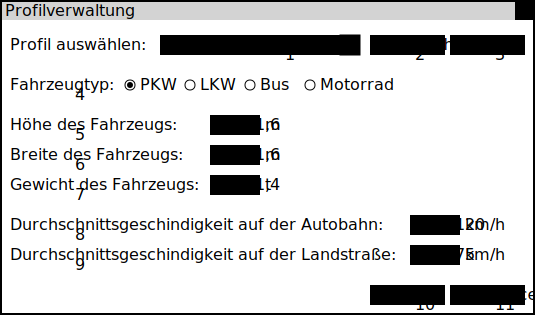
\includegraphics[width=0.9\linewidth]{Profilverwaltung}
\caption{Profilverwaltung}
\label{fig:mockupprofilverwaltung}
\end{figure}
% Betreuer2: Slider für die Zahl? Spinner? (gemacht)
\begin{enumerate}
\item Profil-Auswahl (Combobox, Dropdownmenü):\\
legt ein Profil fest
\item Löschen-Button:\\
löscht das aktuell ausgewählte Profil; bei Standardprofilen deaktiviert (\ref{WF:loescheProfil}); zeigt vorher ein Popup an, das den Nutzer davor warnt, dass er viel Berechnungsarbeit zerstört. 
\item Neu-Button:\\
erstellt eine Kopie des aktuellen Profils; den Namen gibt der Benutzer in einem weiteren Dialog ein (\ref{WF:neuesProfil})
\item Fahrzeugtyp-Auswahl:\\
setzt den Fahrzeugtyp des aktuellen Profils (\ref{D:fahrzeugTyp})
\item Höhen-Eingabe:\\
setzt die Höhe des aktuellen Profils (\ref{D:hoehe})
\item Breiten-Eingabe:\\
setzt die Breite des aktuellen Profils (\ref{D:breite})
\item Gewicht-Eingabe:\\
setzt das Gewicht des aktuellen Profils (\ref{D:gewicht})
\item Autobahn-Geschwindigkeits-Eingabe:\\
setzt die Durchschnittsgeschwindigkeit des aktuellen Profils auf der Autobahn (\ref{D:geschwindigkeitAutobahn})
\item Landstraßen-Geschwindigkeits-Eingabe:\\
setzt die Durchschnittsgeschwindigkeit des aktuellen Profils auf der Landstraße (\ref{D:geschwindigkeitLandstrasse})
\item OK-Button:\\
speichert Änderungen am ausgewählten Profil; setzt es als das aktuelle Profil; schließt den Dialog
\item Abbrechen-Button:\\
verwirft Änderungen am ausgewählten Profil; schließt den Dialog
\end{enumerate}

In diesem Dialog kann der Benutzer Profile hinzufügen, entfernen und bearbeiten, die er im Kartenverwaltung-Dialog (siehe unten, \abbildung{mockupkartenverwaltung}) verschiedenen Karten zuordnen kann. Das Löschen eines Profils mit dem Löschen-Button ist sofort effektiv, Änderungen an einem Profil werden übernommen, sobald der Dialog mit dem OK-Button geschlossen oder in der Profil-Auswahl ein anderes Profil ausgewählt wird.

\subsection{Dialog: Kartenverwaltung}
\begin{figure}[H]
\centering
\includegraphics[width=0.9\linewidth]{Kartenverwaltung}
\caption{Kartenverwaltung}
\label{fig:mockupkartenverwaltung}
\end{figure}
\begin{enumerate}
\item Karten-Auswahl(Combobox, Dropdownmenü):\\
wählt eine Karte aus.
\item Import-Button:\\
fragt den Benutzer nach einer \gls{osm}-Datei und einem Namen; fügt sie in die Karten-Auswahl ein
\item Aktualisieren-Button:\\
fragt den Benutzer nach einer \gls{osm}-Datei; ersetzt die ausgewählte Karte mit dieser
\item Löschen-Button:\\
löscht die ausgewählte Karte aus der Liste
\item Profil-Liste:\\
zeigt am Anfang alle Profile, für die eine \gls{vorberechnung} der ausgewählten Karte existiert
\item Hinzufügen-Button:\\\\
fügt ein Profil zur Profil-Liste der ausgewählten Karte hinzu\\
Zur Profil-Auswahl wird der Profilverwaltung-Dialog gestartet (\abbildung{mockupprofilverwaltung}). Sein OK-Button setzt es nicht als das aktuelle Profil, sondern fügt es stattdessen zur Profil-Liste hinzu.
\item Entfernen-Button:\\
entfernt ein Profil aus der Profil-Liste.
\item OK-Button:\\
übernimmt Änderungen, setzt die ausgewählte Karte als die aktuelle Karte und schließt den Dialog
  \begin{itemize}
  \item Für hinzugefügte Karten wird die \gls{vorberechnung} zum Rendern durchgeführt.
  \item Für aktualisierte Karten werden alle Vorberechnungen (Profile, Rendern) neu durchgeführt.
  \item Für entfernte Karten werden alle Vorberechnungen (Profile, Rendern) gelöscht.
  \item Für zu einer Karte hinzugefügte Profile wird die Vorberechnung durchgeführt.
  \item Für von einer Karte entfernte Profile wird die Vorberechnung gelöscht.
  \end{itemize}
  Bevor diese Aktionen durchgeführt werden, wird dem Benutzer in einem Dialog eine Liste der geplanten Aktionen gezeigt; dabei wird er \emph{eindrücklich} darauf hingewiesen, dass neue Vorberechnungen sehr lange dauern (mit konkretem Zeitraum) und dass gelöschte Vorberechnungen ebenso viel Berechnungsarbeit vernichten.
\item Abbrechen-Button:\\
schließt den Dialog.\\
\end{enumerate}

In diesem Dialog kann der Benutzer Profil-Karten-Kombinationen verwalten. Er kann Karten hinzufügen und entfernen, er kann im Profilverwaltung-Dialog (der erscheint, wenn er den Hinzufügen-Button klickt) Profile hinzufügen und entfernen, und er kann Profil-Karten-Kombinationen hinzufügen und entfernen. Wenn der Benutzer genau die Kombinationen festgelegt hat, die er verwenden möchte, drückt er den OK-Button. Daraufhin wird ihm ein Dialog mit einem Text wie dem folgenden angezeigt:
\begin{quote}
  „Sie haben die folgenden Operationen ausgewählt:
  \begin{itemize}
  \item Hinzufügen der Karte „Baden-Württemberg“
  \item Hinzufügen des Profils „LKW [default]“ zur Karte „Baden-Württemberg“
  \item Entfernen des Profils „PKW [default]“ von der Karte „Karlsruhe“
  \end{itemize}
  Diese Operationen werden etwa \textbf{20 Stunden} benötigen; außerdem wird das Ergebnis von etwa \textbf{10 Stunden} früherer Rechenzeit gelöscht.
  
  Sind Sie sicher, dass sie diese Operationen durchführen wollen?“
\end{quote}
Dabei wird der Dialog bewusst sehr aufdringlich gestaltet, um zu vermeiden, dass der Benutzer aus Versehen die Operationen durchführt; der Bestätigen-Button wird erst nach 5 Sekunden aktiviert.

\subsection{Dialog: Verlauf}
\begin{figure}[H]
\centering
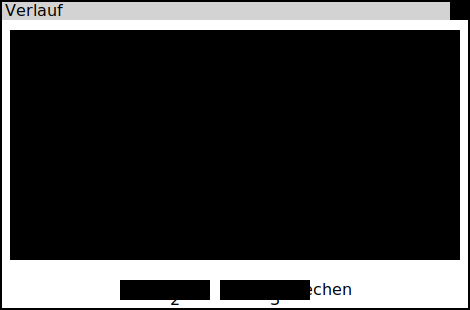
\includegraphics[width=0.7\linewidth]{Verlauf}
\caption{Verlauf}
\label{fig:mockupverlauf}
\end{figure}
\begin{enumerate}
\item Verlauf-Liste:\\
zeigt eine Liste aller \gls{verlauf}-Einträge; der Neueste ganz oben
\item OK-Button:\\
setzt den aktuellen Start- und Zielpunkt nach dem ausgewählten Verlauf-Eintrag; schließt den Dialog
\item Abbrechen-Button:\\
schließt den Dialog
\end{enumerate}

Im Verlauf-Dialog kann der Benutzer frühere Anfragen einsehen und wiederverwenden. Ein einzelner Linksklick auf einen Eintrag wählt diesen Eintrag aus, ein doppelter Linksklick hat den gleichen Effekt wie ein einfacher Linksklick und ein Linksklick auf den OK-Button.
% Fabian

\subsection{Dialog: Über}
\begin{figure}[H]
\centering
\includegraphics[width=0.7\linewidth]{mockup_screenshot_about}
\caption{Über}
\label{fig:mockupabout}
\end{figure}
\begin{enumerate}
\item Informationstext über „routeKIT“
%TODO Genauen Inhalt (gemacht)
\item OK-Knopf:\\
schließt das Fenster
\end{enumerate}

\section{Globale Testfälle und Szenarien}
% Betreuer: Vorbedinung, Aktionen, Nachbedingung (gemacht)
\subsection{Funktionssequenzen}
Bei allen Testfällen gilt als Vorbedingung, dass routeKIT gestartet ist (außer es ist explizit gefordert, dass es gestoppt ist).
%TODO Namen der Testfälle/refs überall einfügen, wo es fehlt (gemacht)
\begin{description}
\itemsep 1em
\subsubsection{Kernfunktionen}
\oitem{TF}{starteVorberechnung} Vorberechnung starten
\testfall[\ref{WK:beschlArc}]
    {Karte ist sichtbar, aktuelles Profil ist nicht vorberechnet (für die aktuelle Karte)}
    {Vorberechnung auswählen, Warnmeldung bestätigen, lange Warten}
    {Aktuelles Profil ist vorberechnet (für die aktuelle Karte)}
% Betreuer2: Wegbeschreibung export testen (gemacht)
\oitem{TF}{wegbeschreibungsexport} Wegbeschreibung exportieren
\testfall[\ref{WK:beschreibung}, \ref{WK:beschreibungExport}]
    {Eine Route mit der Wegbeschreibung ist berechnet}
    {Die Wegbeschreibung wird exportiert}
    {Es liegt eine HTML-Datei mit der Wegbeschreibung vor}
% Betreuer2: Systemstart (gemacht)
\oitem{TF}{systemstart} routeKIT starten
\testfall
    [\ref{MK:karteAnzeigen}, \ref{WK:letztesProfil}, \ref{WK:letzteKarte}]
    {Das Programm ist nicht gestartet}
    {Das Programm wird gestartet}
    {Es wird die zuletzt ausgewählte Karte und das zuletzt ausgewählte Profil geladen (beim ersten Programmstart wird die mitgelieferte Stan\-dard-Kar\-te bzw. das mitgelieferte Standard-Profil für PKWs geladen). Die Karte wird ohne Start- und Zielpunkte und eine berechnete Route angezeigt.}
% Betreuer2: Beenden und neu starten. (gemacht)
\oitem{TF}{exitstartVerlauf} Verlauf nach Neustart
\testfall[\ref{WK:verlauf}]
    {Karte ist sichtbar, aktuelles Profil ist vorberechnet (für die aktuelle Karte)}
    {Der Benutzer wählt Start- und Zielpunkt aus. Das Programm wird beendet. Das Programm wird gestartet.}
    {Im Verlauf befindet sich ein Eintrag für die vorher berechnete Route}
\oitem{TF}{ladeRoute} Route aus Verlauf laden
\testfall
    [\ref{WK:verlauf}]
    {Eine Route wurde bereits berechnet, die Route wird nicht angezeigt}
    {Die Route wird aus dem Verlauf geladen}
    {Die abgespeicherte Route wird angezeigt}
\oitem{TF}{exitstartBerechnung} Vorberechnung nach Neustart
\testfall[\ref{D:vorberechnung}]
    {Karte ist sichtbar, aktuelles Profil ist nicht vorberechnet (für die aktuelle Karte)}
    {Der Benutzer führt die Vorberechnung aus, beendet das Programm, startet das Programm}
    {Das zuvor berechnete Profil ist immer noch berechnet (für die aktuelle Karte)}
\oitem{TF}{exportGPX} GPX-Export
\testfall[\ref{WK:routeExport}]
    {Karte ist sichtbar, aktuelles Profil ist vorberechnet (für die aktuelle Karte), Eine Route wird angezeigt}
    {Der GPX Exportvorgang wird durchgeführt.}
    {Es ist eine valide GPX-Datei mit der berechneten Route vorhanden.}
\subsubsection{GUI Tests}
\oitem{TF}{waehleErstenPunkt} Ersten Punkt wählen
\testfall
	[\ref{MK:startZielWaehlen}, \ref{MK:startZielZeigen}]
    {Karte ist sichtbar, Profil ist vorberechnet (für die aktuelle Karte)}
    {Auswählen des Start- bzw. Zielpunkts}
    {Start- bzw. Zielpunkt ist ausgewählt und wird auf der Karte angezeigt}
\oitem{TF}{waehleZweitenPunkt} Zweiten Punkt wählen
\testfall
    [\ref{MK:routeBerechnen}, \ref{MK:routeAnzeigen}]
    {Karte ist sichtbar, Profil ist vorberechnet (für die aktuelle Karte),  Start- oder Zielpunkt ist ausgewählt (\ref{TF:waehleErstenPunkt})}
    {Auswählen des anderen Punkts (Ziel- bzw. Startpunkts)}
    {Route für die Angaben ist berechnet und wird angezeigt}
\oitem{TF}{waehlePunktErneut} Punkt erneut wählen
\testfall
    [\ref{MK:routeBerechnen}, \ref{MK:routeAnzeigen}]
    {Karte ist sichtbar, Profil ist vorberechnet (für die aktuelle Karte),  Start- und Zielpunkt sind ausgewählt}
    {Erneutes Auswählen des  Ziel- oder Startpunkts}
    {Route für die neuen Angaben ist berechnet und wird angezeigt}
\oitem{TF}{zieheKarte} Karte ziehen
\testfall
    [\ref{MK:karteVerschieben}]
    {Karte ist sichtbar}
    {Ziehen der Karte}
    {Der angezeigte Kartenausschnitt hat sich entsprechend verändert}
    %FIXME Klingt irgendwie seltsam... ne, (gemacht)
\oitem{TF}{zoomeRein} Reinzoomen
\testfall
    [\ref{MK:karteZoomen}]
    {Karte ist sichtbar}
    {Reinzoomen}
    {Ein Ausschnitt der Karte wird größer und genauer dargestellt}
\oitem{TF}{zoomeRaus} Rauszoomen
\testfall
    [\ref{MK:karteZoomen}]
    {Karte ist sichtbar}
    {Rauszoomen}
    {Ein größerer Bereich der Karte wird angezeigt}
\oitem{TF}{verbieteWaehlePunkt} Punkt wählen ohne Vorberechnung
\testfall
    {Karte ist sichtbar, aktuelles Profil ist nicht vorberechnet (für die aktuelle Karte)}
    {Versuchen Start- bzw. Zielpunkte auszuwählen}
    {Kein Start- oder Zielpunkt ist ausgewählt} % Betreuer2: Meldung, Popup nicht gut?, StatusBar (gemacht: Keine Meldung großer Knopf.)
\oitem{TF}{geocoords} \gls{dezimalkoordinaten} eingeben
\testfall[\ref{WK:koordinaten}]
    {Karte ist sichtbar, Profil ist vorberechnet (für die aktuelle Karte)}
    {Der Benutzer tippt Start- oder Zielkoordinaten als \gls{dezimalkoordinaten} ein}
    {Die Start- oder Zielkoordinaten sind nun auf die angegebenen abgeändert, Start- oder Zielpunkt wird angezeigt}
\oitem{TF}{guideleteprofile} \gls{standardprofil} löschen
\testfall[\ref{WK:standardprofile}]
    {Es wurde das Fenster zur Profil-Verwaltung geöffnet.}
    {Ein mitgeliefertes Standard-Profil wird ausgewählt.}
    {Der Knopf zum Löschen des Profils wird deaktiviert.}
\oitem{TF}{guideletemap} Standard-Karte löschen
\testfall
    {Es wurde das Fenster zur Karten-Verwaltung geöffnet.}
    {Eine mitgelieferte Standard-Karte wird ausgewählt.}
    {Der Knopf zum Löschen der Karte wird deaktiviert.}
\oitem{TF}{osmKacheln} \glspl{osmkachel} verwenden
\testfall[\ref{WK:osmKacheln}]
    {Karte ist sichtbar, Internetverbindung ist hergestellt}
    {Wechseln der Darstellungs-Art auf \glspl{osmkachel}}
    {Die Karte wird mit \glspl{osmkachel} angezeigt}
\oitem{TF}{eigeneKacheln} Eigene Kacheln verwenden
\testfall[\ref{MK:karteAnzeigen}, \ref{MK:karteRendern}]
    {Karte ist sichtbar, OSM-Render-Modus ist aktiviert}
    {Wechseln der Darstellungs-Art auf „eigene Kacheln“}
    {Die Karte wird mit selbst gerenderten Kacheln angezeigt,
    es ist keine Internetverbindung mehr nötig (um die Karte zu verschieben oder zu zoomen)}
\oitem{TF}{placeholder} Placeholder-Kacheln
\testfall[\ref{WK:kartePlaceholder}]
    {Karte ist sichtbar}
    {Die Karte schnell bewegen oder zoomen}
    {Das Programm hängt nicht, stattdessen werden graue Kacheln angezeigt, die nach kurzer Zeit durch die richtigen Kacheln ersetzt werden}
\subsubsection{Profilverwaltung}
\oitem{TF}{profilAnlegen} Profil anlegen
\testfall
    [\ref{WK:profilerstellen}]
    {–}
    {Neues Profil anlegen}
    {Das neue Profil ist ausgewählt, das neue Profil ist nicht vorberechnet (für die aktuelle Karte)}
\oitem{TF}{waehleProfil} Profil auswählen
\testfall[\ref{WK:profile}]
    {Ein Profil ist vorhanden und nicht ausgewählt}
    {Das Profil wird ausgewählt}
    {Das Profil ist ausgewählt}
\oitem{TF}{loescheProfil} Profil löschen
\testfall
    [\ref{WK:profilloeschen}]
    {Ein Profil, das nicht das Standardprofil ist, ist vorhanden}
    {Das Profil wird gelöscht}
    {Das Profil ist nicht mehr vorhanden}
\oitem{TF}{aendereProfil} Profil ändern
\testfall
    [\ref{WK:profilaendern}]
    {Ein Profil ist vorhanden}
    {Das Profil wird geändert, die Profilverwaltung geschlossen und wieder geöffnet}
    {Das Profil hat immer noch die neuen Daten}
\oitem{TF}{profilPersistenz} Profil ändern und Neustart
\testfall
    {Ein Profil ist vorhanden}
    {Das Profil wird geändert, das Programm wird geschlossen, das Programm wird geöffnet}
    {Die Änderungen sind immer noch vorhanden}
\oitem{TF}{routeNeuBerechnenProfil} Neuberechnen der Route bei Profiländerung
\testfall[\ref{WK:routeNeuBerechnenProfil}]
    {Karte ist sichtbar, eine Route wurde berechnet}
    {Das Profil wird geändert}
    {Die berechnete Route wird mit den neuen Daten aus dem ausgewähltem Profil neu berechnet}
\subsubsection{Kartenverwaltung}
\oitem{TF}{importKarte} Karte importieren
\testfall[\ref{WK:karteImportiere}]
    {–}% Betreuer2: ganz weg (gemacht)
    {Eine neue Karte wird importiert}
    {Die neue Karte ist ausgewählt, die Karte ist für das aktuelle Profil nicht vorberechnet}
\oitem{TF}{wechsleKarte} Karte auswählen
\testfall[\ref{WK:karteAuswaehlen}]
    {Eine Karte ist ausgewählt}
    {Eine andere Karte wird ausgewählt}
    {Die andere Karte ist ausgewählt}
\oitem{TF}{loescheKarte} Karte löschen
\testfall[\ref{WK:karteLoeschen}]
    {Eine andere Karte als die Standardkarte ist vorhanden}
    {Die Karte wird gelöscht}
    {Die Karte ist nicht mehr vorhanden}
\oitem{TF}{kartenPersistenz} Karte importieren und Neustart
\testfall
    {-}
    {Eine Karte wird importiert, das Programm wird geschlossen, das Programm wird geöffnet}
    {Die neue Karte ist immer noch vorhanden}
\oitem{TF}{routeLoeschenKarte} Löschen der Route bei Kartenänderung
\testfall[\ref{WK:routeLoeschenKarte}]
    {Karte ist sichtbar, eine Route wurde berechnet}
    {Die Karte wird geändert}
    {Die berechnete Route wird verworfen}
\subsubsection{Beschränkungen}
\oitem{TF}{einbahnstrasse} Einbahnstraße – Ende-zu-Ende
\testfall[\ref{WK:einbahnstrasse}]
    {Karte ist sichtbar, Profil ist vorberechnet (für die aktuelle Karte), Karte enthält eine Einbahnstraße}
    {Als Startpunkt wird das Ende und als Ziel der Anfang der Einbahnstraße ausgewählt}
    {Ein Weg, der nicht diese Einbahnstraße enthält, wird gefunden}
\oitem{TF}{einbahnstrasseHard} Einbahnstraße – innerhalb (Randfall für \gls{dijkstra})
\testfall[\ref{WK:einbahnstrasse}]
    {Karte ist sichtbar, Profil ist vorberechnet (für die aktuelle Karte), Karte enthält eine Einbahnstraße}
    {Als Start- und Zielpunkt werden Punkte auf der Einbahnstraße gewählt. Dabei ist Start weiter in Einbahnstraßenrichtung als Ziel.}
    {Ein Weg, der die Einbahnstraße nicht entgegen der Fahrtrichtung benutzt, wird gefunden}
\oitem{TF}{abbiegebeschraenkung} Abbiegebeschränkung
\testfall[\ref{WK:abbiegebeschraenkung}]
    {Karte ist sichtbar, Profil ist vorberechnet (für die aktuelle Karte), Karte enthält eine Abbiegebeschränkung}
    {Startpunkt auf die Straße, von der nicht abgebogen werden darf, setzen. Zielpunkt auf die Straße, in die nicht abgebogen werden darf, setzen. }
    {Ein Weg, der diesen Abbiegevorgang nicht enthält, wird gefunden}
\oitem{TF}{einschraenkungNeg} Beschränkung trifft zu
\testfall
    {Karte ist sichtbar, Profil ist vorberechnet (für die aktuelle Karte), Karte enthält eine Höhen-, Breiten- oder Gewichtsbeschränkung, im aktuellen Profil ist ein größerer Wert dafür angegeben}
    {Als Startpunkt wird der Anfang und als Ziel das Ende der Straße mit Beschränkung ausgewählt}
    {Ein Weg, der diese Straße nicht enthält, wird gefunden}
\oitem{TF}{einschraenkungPos} Beschränkung trifft nicht zu
\testfall
    {Karte ist sichtbar, Profil ist vorberechnet (für die aktuelle Karte), Karte enthält eine Höhen-, Breiten- oder Gewichtsbeschränkung, im aktuellen Profil ist ein kleinerer Wert dafür angegeben}
    {Als Startpunkt wird der Anfang und als Ziel das Ende der Straße mit Beschränkung ausgewählt}
    {Die beschränkte Straße wird als Route gefunden}
\oitem{TF}{typEinschraenkungNeg} Typ-Einschränkung trifft zu
\testfall[\ref{WK:fahrzeugtyp}]
    {Karte ist sichtbar, Profil ist vorberechnet (für die aktuelle Karte), Karte enthält eine Beschränkung für einen Fahrzeugtyp, im aktuellen Profil ist dieser Typ angegeben}
    {Als Startpunkt wird der Anfang und als Ziel des Ende der Straße mit Beschränkung ausgewählt}
    {Ein Weg, der diese Straße nicht enthält, wird gefunden}
\oitem{TF}{typEinschraenkungPos} Typ-Einschränkung trifft nicht zu
\testfall[\ref{WK:fahrzeugtyp}]
    {Karte ist sichtbar, Profil ist vorberechnet (für die aktuelle Karte), Karte enthält eine Beschränkung für einen Fahrzeugtyp, im aktuellen Profil ist ein anderer Fahrzeugtyp angegeben}
    {Als Startpunkt wird der Anfang und als Ziel des Ende der Straße mit Beschränkung ausgewählt}
    {Die beschränkte Straße wird als Route gefunden}

% Betreuer2: Keine Interpretation (gemacht)
% Betreuer2: Gruppieren (gemacht)
% Betreuer2: Route anzeigen und Profil ändern (gemacht)
% Betreuer2: Mehr Beschränkungstests (gemacht)
% Betreuer2: kein beinhalten (gemacht)

% Betreuer2: Karten/Kartendaten/Profil Begriff, Karte ^= Anschauen
% Betreuer2: Renderer ändern im GUI (gemacht)


\end{description}
\subsection{Testszenarien}
% Betreuer2: Testszenarien (gemacht)
% ersterStart, programmnutzung: verified by Lucas
%TODO Verify
\begin{description}
\oitem{TS}{ersterStart} Erster Start\\
Alice startet das Programm routeKIT zum ersten Mal. Nach einem Ladevorgang sieht sie eine eine Karte von Karlsruhe (\abbildung{mockupscreenshotmain}). Alice kann zwischen zwei Standardprofilen wählen, wobei eines für \glspl{pkw} und das andere für \glspl{lkw} ist.
Sie wählt das Profil „PKW [default]“. Sie verschiebt die Karte, indem sie die linke Maustaste gedrückt hält, und zoomt die Karte mit den Zoom-Buttons, bis sie die Hebelstraße findet. 
Mit einem Rechtsklick öffnet sie das Kontextmenü und wählt diesen Punkt als Startpunkt. Die Koordinaten des Startpunkts werden in dem dafür vorgesehen Feld angezeigt. Um den Zielpunkt auszuwählen, tippt Alice in das Feld „Ziel“ die \gls{dezimalkoordinaten} \texttt{49,01386 8,38106} ein. 
Auf der Karte wird ein Punkt als Ziel markiert und die kürzeste Route zwischen dem Start- und dem Zielpunkt wird auf der Karte angezeigt. Im Feld der Textbeschreibung erscheinen textuelle Anweisungen für die angezeigte Route. Alice wählt den Menüpunkt „Export“ und es erscheinen die Unterpunkte „Route (GPX)\ldots“ und  „Beschreibung (HTML)\ldots“ (\abbildung{mockupscreenshotmenu}). Alice drückt auf  „Beschreibung (HTML)\ldots“ und es wird eine Datei mit der Beschreibung erstellt. Alice schließt das Programm.


\oitem{TS}{programmnutzung} Programmnutzung\\
Alice’ Computer hat eine Internetverbindung. Alice startet das Programm routeKIT. Nach einem Ladevorgang sieht sie die zuletzt verwendete Karte. Das zulezt verwendete \gls{profil} ist ausgewählt. Alice drückt auf den „Profil-Button“ und ein Fenster „Profilverwaltung“  (\abbildung{mockupprofilverwaltung}) erscheint. Sie wählt zwischen den erstellten Profilen das \gls{profil} „Mein PKW“ und drückt den „Löschen-Button“. Es erscheint ein Popup mit der Frage „Wollen sie das Profil wirklich löschen?“. Alice drückt auf „Ja“. Dann wählt sie das Profil „MeinLKW“ und drückt auf „OK“. Sie drückt den „Karten-Button“ und es wird das Fenster „Kartenverwaltung“ (\abbildung{mockupkartenverwaltung}) angezeigt. Alice wählt die Karte „Hamburg“ aus und drückt den „Löschen-Button“. Sie drückt „OK“. Es erscheint eine Warnung, dass durch den Löschvorgang wichtige Daten gelöscht werden, die mehrere Stunden Berechnung benötigt haben. Alice drückt „OK“ und die Karte ist gelöscht. Jetzt wählt Alice die Karte „Karlsruhe“ aus und drückt „OK“. Sie drückt den „Verlauf-Button“ und der Verlauf wird angezeigt. Alice wählt den obersten Eintrag aus und drückt auf „OK“. Die \gls{route} wird auf der Karte angezeigt. Im Feld der Textbeschreibung erscheinen textuelle Anweisungen für die angezeigte Route. Alice exportiert die Route als GPX-Datei (\abbildung{mockupscreenshotmenu}). Alice wählt den Menüpunkt „Verwaltung“ und es erscheinen die Unterpunkte „Profile\ldots“, „Karten\ldots“ und  eine Checkbox „OSM-Renderer verwenden“. Alice fordert die \glspl{osmkachel} an. Die Darstellung der Karte verändert sich. Alice verwendet den „Start/Ziel-tauschen-Button“. Die \gls{route} wird neu berechnet und angezeigt. Alice wählt den Menüpunkt „routeKIT“ und den Unterpunkt „Über\ldots“ aus. Sie drückt auf „OK“. Alice wählt den Menüpunkt „routeKIT“ und den Unterpunkt „Beenden“ aus.

\oitem{TS}{verwaltung} Verwaltung\\
Der Administrator einer Firma möchte routeKIT auf allen Rechnern der Firma installieren. Allerdings sind die \glspl{standardprofil} und die mitgelieferte Karte nicht für alle Benutzer geeignet; deshalb möchte der Administrator eigene Profile und Karten erstellen.

Der Administrator startet zunächst routeKIT und öffnet den Kartenverwaltungs-Dialog (\abbildung{mockupkartenverwaltung}) und importiert eine Deutschlandkarte, da die Firma deutschlandweit operiert; für eine Außenstelle in Bielefeld importiert er außerdem eine Bie\-le\-feld-Kar\-te. Dann entfernt er die Standardprofile von allen Karten und fügt stattdessen eigene Profile hinzu. Beim Klicken auf den Hinzufügen-Button öffnet sich der Profilverwaltungs-Dialog (\abbildung{mockupprofilverwaltung}); hier erstellt er zunächst die Profile, die die Firma benötigt:
\begin{itemize}
\item Firmenauto: Ein \gls{pkw}, der etwas leichter und langsamer ist als das Standardprofil
\item Boss-Auto: Der Boss fährt einen schnellen Mercedes
\item Firmenlaster: Ein \gls{lkw}, der auf der Autobahn noch langsamer ist als das Standardprofil
\item Mannis Laster: Ein getuneter \gls{lkw}, der schwerer beladen wird als normale \gls{lkw}
\end{itemize}
Dann schließt der Administrator den Profilverwaltungs-Dialog und ordnet diese Profile den Karten zu:
\begin{itemize}
\item In Karlsruhe werden das Firmenauto und das Boss-Auto verwendet
\item In Bielefeld wird nur das Firmenauto verwendet
\item Die Laster sind deutschlandweit unterwegs
\end{itemize}
Wenn der Administrator mit den Änderungen zufrieden ist, drückt er den OK-Button. In einem Dialog wird er nochmal über die Änderungen informiert. Hier sieht er, dass er versehentlich das Boss-Auto zur Bielefelder Außenstelle hinzugefügt hat; er drückt „Abbrechen“ und entfernt das Boss-Auto aus der Bielefeld-Karte und klickt erneut OK. Diesmal ist er mit den Änderungen zufrieden; er schickt seinem Vorgesetzten eine Nachricht mit der geschätzten Berechnungszeit und startet dann die Berechnung, indem er den OK-Button drückt. Eine Woche später installiert er das Programm mit den eingerichteten Karten und Profilen auf den Rechnern aller Mitarbeiter.

\end{description}

\subsection{Datenkonsistenzen}

\begin{description}
\oitem{TD}{datenProfilVorberechnung}
Eine Route kann nur berechnet werden, wenn \gls{kartendaten} vorliegen, ein \gls{profil} ausgewählt wurde und die \gls{vorberechnung} für dieses \gls{profil} für diese Karte abgeschlossen ist.
\oitem{TD}{gültigOsm}
\gls{kartendaten} müssen als gültige \gls{osm}-Datei vorliegen.
\oitem{TD}{karteProfilGelöscht}
Eine gespeicherte Route kann nicht angezeigt werden, wenn die zugehörigen Kartendaten und das verwendete \gls{profil} nicht mehr vorhanden sind.
\oitem{TD}{löscheNichtStandard}
Das \gls{standardprofil} kann nicht gelöscht werden.
\oitem{TD}{profil}
Es ist ein \gls{profil} ausgewählt.
\oitem{TD}{karte}
Es ist eine Karte ausgewählt.
\end{description}
% Fabian
\section{Entwicklungsumgebung}
\begin{description}
\item[Teamkommunikation] E-Mail-Verteiler, Skype
\item[Dokumentation] \LaTeX{}
\item[UML-Planungswerkzeug] UMLet
\item[IDE] Eclipse
\item[Qualitätssicherung] JUnit, CodeCover
\item[Versionskontrolle] Git
\end{description}
% Kevin

\glsaddallunused
\makeatletter
\newglossarystyle{myAltlist}{
  \glossarystyle{altlist} % base this style on altlist
  \renewcommand*{\glossaryentryfield}[5]{
  \item[\glsentryitem{##1}\glstarget{##1}{##2}]
    \mbox{}\par\nobreak\@afterheading
    ##3\glspostdescription\space Auf Seite ##5.
  }
}
\makeatother
\printglossary[type=main, title={Glossar}, toctitle={Glossar}, style=myAltlist]

\end{document}
